\documentclass{article}

\usepackage{arxiv}
\usepackage[utf8]{inputenc}
\usepackage[T1]{fontenc}
\usepackage{hyperref}
\usepackage{url}
\usepackage{booktabs}
\usepackage{amsfonts}
\usepackage{nicefrac}
\usepackage{microtype}
\usepackage{graphicx}
\usepackage{natbib}
\usepackage{doi}
\usepackage{fancyhdr}
\usepackage{tikz}
\usepackage{pgfplots}

\title{Parallel-CPU-based-Shortest-Path-in-Graph-Algorithms}
\date{December 1, 2025}

% Uncomment to override  the `A preprint' in the header
%\renewcommand{\headeright}{Technical Report}
%\renewcommand{\undertitle}{Technical Report}
\renewcommand{\shorttitle}{Parallel SSSP Algorithms}

\hypersetup{
  pdftitle={Parallel-CPU-based-Shortest-Path-in-Graph-Algorithms},
  pdfsubject={Parallel Algorithms, shortest path},
  pdfauthor={Isaac Shepherd, <Coauthor Name>},
  pdfkeywords={SSSP, Dijkstra, Bellman-Ford, Delta-Stepping, MPI, OpenMP, pthreads, Parallel Computing},
}

\author{
    Isaac Shepherd \\
	University of Texas at Austin \\
    is23423@my.utexas.edu \\
    \And
    <Author 2 Name> \\
    <Affiliation 2> \\
    <Email 2> \\
    % Add more authors as needed
}

\pagestyle{fancy}
\fancyfoot[C]{\thepage}

\begin{document}
\maketitle

\begin{abstract}
A comparative study of single-source shortest path algorithms (Dijkstra, Bellman-Ford, Delta-Stepping) implemented using MPI, pthreads, and OpenMP. 
Experiments on large DIMACS graph demonstrate the strengths and weaknesses of each approach in terms of scalability and performance. 
Results show that Bellman-Ford scales well on distributed systems, Delta-Stepping provides a brief increase in performance but degrades at higher thread counts, and Dijkstra's algorithm exhibits poor scalability due to its inherently sequential global minimum selection process.
Results provide practical guidance for selecting parallel SSSP algorithms on parallelism models (MPI, OpenMP, pthreads) for graph processing.
\end{abstract}

\keywords{Single-source shortest path \and Dijkstra \and Bellman-Ford \and Delta-Stepping \and MPI \and OpenMP \and pthreads \and Parallel algorithms}

\section{Introduction}
Single-source shortest path (SSSP) algorithms are fundamental in graph theory with widespread applications in fields such as networking, transportation, and scientific engineering. 
As graphs representing real-world applications grow in size and complexity, efficient parallelization of SSSP algorithms becomes increasingly necessary to achieve practical performance. 
In this project, we compare three classic SSSP algorithms—Dijkstra, Bellman-Ford, and Delta-Stepping—implemented using three parallel programming models: MPI, pthreads, and OpenMP. 
The goal is to evaluate the scalability and efficiency of each approach on the `internet.egr` DIMACS benchmark graph, which consists of 124,651 nodes and 387,240 edges and represents a snapshot of the world internet topology at the autonomous systems level. 
These tests provide insights into the strengths and limitations of different parallelization strategies for high-performance graph processing.

\section{Background}

The single-source shortest path (SSSP) problem is a foundational problem in graph theory, with applications ranging from network routing, transportation planning, and scientific simulations. 
Given a weighted graph and a source node, the goal is to find the shortest path from the source to every other node in the graph.

Several classic algorithms have been developed to solve the SSSP problem. 
\textbf{Dijkstra's algorithm} is an aglorithm published in 1959 by Edsger W. Dijkstra, efficient for graphs with non-negative edge weights and is widely used due to its optimality and simplicity. 
However, it is inherently sequential because it relies on selecting a global minimum distance node at each step. 
\textbf{Bellman-Ford's algorithm} is an algorithm published in 1958 by Richard Bellman and Lester Ford that can handle graphs with negative edge weights and is more amenable to parallelization, as it relaxes all edges in each iteration. 
\textbf{Delta-Stepping} is a more recent algorithm designed in 1998 by Ulrich Meyer and Peter Sanders, to combine the advantages of Dijkstra and Bellman-Ford, offering better parallel scalability by processing nodes in "buckets" based on distance ranges.

With the increasing size of real-world graphs, parallel computing has become essential for practical SSSP computation. Three major parallel programming models are commonly used: 
\textbf{MPI} (Message Passing Interface) for distributed-memory systems, \textbf{pthreads} for shared-memory multi-threading, and \textbf{OpenMP} for high-level shared-memory parallelism. 
Each model presents unique challenges and opportunities for parallelizing SSSP algorithms.

This project builds on these foundations by implementing and comparing Dijkstra, Bellman-Ford, and Delta-Stepping algorithms using MPI, pthreads, and OpenMP, and evaluating their performance on a large, real-world internet topology graph.

\section{Methods}

To establish a baseline for performance and correctness, we first implemented sequential versions of the three single-source shortest path algorithms: Dijkstra, Bellman-Ford, and Delta-Stepping. Each algorithm was written in C++ and tested on the same large DIMACS graph (`internet.egr`) to ensure consistent input and output formats across all experiments.

\textbf{Dijkstra's algorithm} was implemented using a min-heap (priority queue) to select the node with the smallest tentative distance at each step. 
This version is suitable for our graph with no negative edge weights, and serves as a reference for optimal sequential performance.

\textbf{Bellman-Ford's algorithm} was implemented in its classic form, relaxing all edges in the graph for each of $(n-1)$ iterations, where $n$ is the number of nodes. 
This approach can handle negative edge weights and is capable of detecting negative-weight cycles, however we omitted negative-weight cycle detection in our implementation as the input graph is known to have no such cycles.

\textbf{Delta-Stepping} was implemented as a bucket-based algorithm, dividing nodes into buckets according to their tentative distances. 
The algorithm alternates between relaxing "light" edges (with weights less than or equal to a chosen $\delta$ parameter) and "heavy" edges (with weights greater than $\delta$). 
The $\delta$ parameter was set to ten times the average edge weight of the input graph ($\delta = 10 \times \text{avg. edge weight}$) for all experiments, as this value provided balance between parallelism and synchronization overhead in practice.

To compare the baseline performance of the three algorithms, we measured the runtime of each sequential implementation on the \texttt{internet.egr} graph. The results are shown in Figure~\ref{fig:seq-sssp-times}.
\begin{figure}[ht]
    \centering
    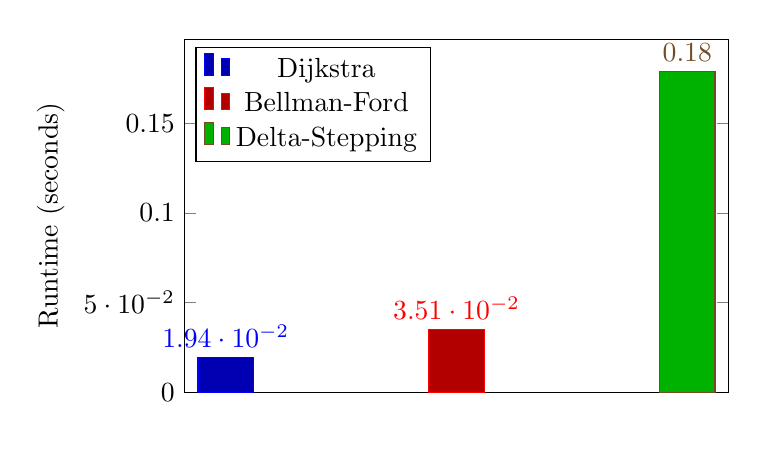
\begin{tikzpicture}
        \begin{axis}[
            ybar,
            bar width=20pt,
            ylabel={Runtime (seconds)},
            symbolic x coords={Dijkstra, Bellman-Ford, Delta-Stepping},
            xtick=data,
            xtick style={draw=none},
            xticklabels={},
            nodes near coords,
            ymin=0,
            width=0.7\textwidth,
            height=0.5\textwidth,
            enlarge x limits=0.3,
            legend style={at={(0.02,0.98)},anchor=north west}
        ]
        \addplot+[ybar, fill=blue!70!black] coordinates {(Dijkstra, 0.0194)};
        \addplot+[ybar, fill=red!70!black] coordinates {(Bellman-Ford, 0.0351)};
        \addplot+[ybar, fill=green!70!black] coordinates {(Delta-Stepping, 0.1788)};
        \legend{Dijkstra, Bellman-Ford, Delta-Stepping}
        \end{axis}
    \end{tikzpicture}
    \caption{Sequential runtime comparison of Dijkstra, Bellman-Ford, and Delta-Stepping algorithms on the \texttt{internet.egr} graph.}
    \label{fig:seq-sssp-times}
\end{figure}

As shown in Figure~\ref{fig:seq-sssp-times}, Dijkstra's algorithm achieved the fastest sequential runtime, followed by Bellman-Ford, with Delta-Stepping being the slowest. 
This ordering is expected, Dijkstra's algorithm is highly efficient for graphs with non-negative edge weights due to its use of a priority queue and greedy selection of the minimum-distance nodes. 
While Bellman-Ford is more flexible in handling negative weights, it incurs additional overhead computation by relaxing all edges in each iteration. 
Although Delta-Stepping is designed for parallel efficiency, it introduces extra overhead in the sequential case from managing buckets and additional data structures, which makes it less efficient than the other two algorithms when run on a single thread. 
These results provide a baseline for evaluating the impact of parallelization in the following sections.

\section{Results}
% Experimental results, tables, and figures.

\section{Discussion}
% Analysis and discussion of results.

\section{Conclusion}
% Conclusion and future work.

\bibliographystyle{unsrtnat}
\bibliography{references}

\end{document}